\documentclass{standalone}
\usepackage{pgfplots}
\definecolor{navy}{rgb}{0,0,0.55}
\definecolor{ruby}{rgb}{0.78,0.15,0.21}
\definecolor{bottle}{rgb}{0.11,0.64,0.22}
\begin{document}
\pgfplotsset{ticks=none}
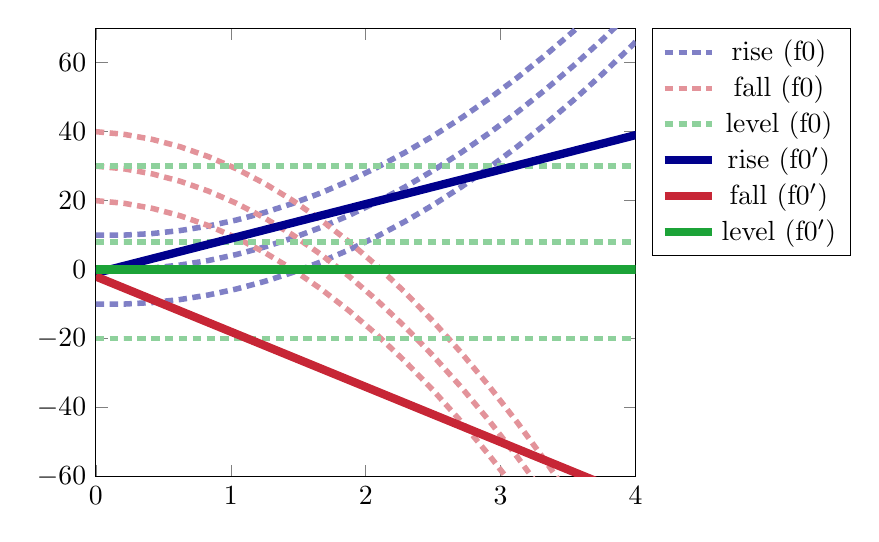
\begin{tikzpicture}
\begin{axis}[no markers, legend pos=outer north east, domain=0:5, ymin=-60,
  ymax=70, xmin=0, xmax=4, legend entries={rise (f0),,,fall
    (f0),,,level (f0),,,
    rise (f0$'$), fall (f0$'$), level (f0$'$)}]
\addplot [line width=2pt, densely dashed, navy!50] {5*x^2-x};
\addplot [line width=2pt, densely dashed, navy!50] {5*x^2-x+10};
\addplot [line width=2pt, densely dashed, navy!50] {5*x^2-x-10};
\addplot [line width=2pt, densely dashed, ruby!50] {-8*x^2-2*x+40};
\addplot [line width=2pt, densely dashed, ruby!50] {-8*x^2-2*x+20};
\addplot [line width=2pt, densely dashed, ruby!50] {-8*x^2-2*x+30};
\addplot [line width=2pt, densely dashed, bottle!50] {-20};
\addplot [line width=2pt, densely dashed, bottle!50] {30};
\addplot [line width=2pt, densely dashed, bottle!50] {8};
\addplot [line width=3pt, navy] {10*x-1};
\addplot [line width=3pt, ruby] {-16*x-2};
\addplot [line width=3pt, bottle] {0};
%\addplot [black] {((x+0.01)^3-(x)^3)/0.01};
\end{axis}
\end{tikzpicture}

\end{document}